\documentclass[article,12pt,openright,oneside,a4paper,brazil]{abntex2}
\usepackage[utf8]{inputenc}
\usepackage{graphicx}
\usepackage{subfig}
\usepackage{lmodern}
\usepackage{float}
\usepackage[brazil]{babel}
\usepackage{booktabs}
\usepackage{longtable}
\usepackage{setspace}
\usepackage{parskip}
\usepackage{leading}
\usepackage{amsmath,esint}
\usepackage{amssymb}
\usepackage{physics}
\usepackage{indentfirst}
\usepackage{gensymb}

\renewcommand{\ABNTEXchapterfont}{\fontfamily{cmr}\fontseries{b}\selectfont}
%%\renewcommand{\ABNTEXchapterfontsize}{\LARGE}

\titulo{Difração de raios X}
\autor{
    \makebox[.6\textwidth]{
    	Gabriel Cardoso de Mello \hfill 
        RA:	21024215}\\
	\makebox[.6\textwidth]{
    	Guilherme Fortes Evangelista \hfill
        RA: 21062515}\\
	\makebox[.6\textwidth]{
    	Letícia de Freitas Santos \hfill 
        RA: 11084215}\\
    \makebox[.6\textwidth]{
    	Rodrigo dos Santos Pereira\hfill 
        RA: 11095516}\\}
\instituicao{Universidade Federal do ABC}
\local{Santo André}
\tipotrabalho{Relatório}
\orientador{Lucas Almeida Miranda Barreto\\}
\date{Abril de 2019}

\renewcommand{\imprimircapa}{%
\begin{capa}%
	\begin{figure}[ht]
		\centering
		
\includegraphics[scale=0.6]{logo.jpg}
		\label{fig:logo}
	\end{figure}
	\begin{center}
		\textbf{\large Laboratório de Física III - BC1419}
		\vfill
    	{\LARGE\textbf{\imprimirtitulo}}
    	\vfill
    	Docente: \imprimirorientador
    	\vspace*{1cm}
		\imprimirautor
		\vfill
    	\imprimirlocal \\
    	\imprimirdata
	\end{center}
\end{capa}
}

\setlength{\parindent}{1.3cm}
\setlength{\parskip}{0.2cm}

\begin{document}
\begin{KeepFromToc}
\imprimircapa
\tableofcontents
\end{KeepFromToc}
\newpage
\begin{abstract}
    A técnica de difração de raios X é muito utilizada na cristalografia por possibilitar a caracterização de materiais tanto orgânicos quanto inorgânicos. No presente trabalho foram realizadas medidas de difração em monocristais de KBr e LiF com o anodo de Cu para verificar o padrão de difração dessas amostras, bem como investigar a radiação contínua e característica em função da tensão aplicada e como minimizar as linhas espectrais k$_\alpha$ e k$_\beta$ com filtros de Ni e Cu.
\end{abstract}

\newpage
\pagenumbering{arabic}
\section{Introdução}\textual

Wihelm Conrad Rontgen foi o físico alemão que descobriu e deu início aos estudos os raios X em 1895. Os raios X são radiações eletromagnéticas na ordem de $10^{-2}$ a $10$ nm e são produzidos quando elétrons em altas velocidades são chocados contra um alvo metálico. Um tubo de raios X é composto de um anodo e um catodo. O catodo, que é um filamento, emite um feixe de elétrons em algumas dezenas de KeV em direção ao alvo ou anodo. A perda brusca de energia devida às repetidas colisões dos elétrons com os átomos do alvo origina o espectro contínuo de raios X, além de uma parte da energia se transformar em calor. Quando um elétron acelerado interage com um átomo, isto é, arranca um elétron de uma camada mais interna e, outro elétron de uma camada mais externa pula para preencher a lacuna na camada anterior, é emitido um fóton de raio X, cuja energia é característica do anodo, pois depende do número atômico do elemento que o compõe. A radiação característica é composta por duas linhas espectrais k$_\alpha$ e k$_\beta$, que correspondem, respectivamente, à transição entre as camadas L para a K e da M para a K.
 
\begin{figure}[H]
    \centering
    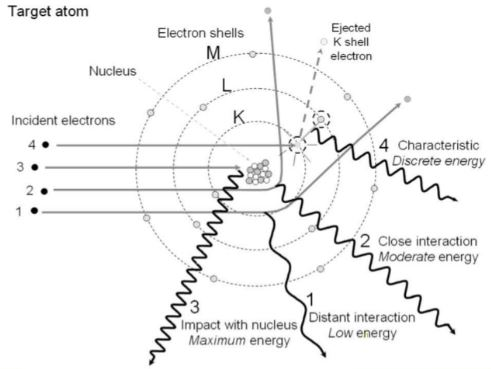
\includegraphics[scale=0.7]{Figuras/raiosX.jpg}
    \caption{Esquema da formação de um fóton de raio X. Fonte: SEIBERT, J. Anthony. X-ray imaging physics for nuclear medicine technologists. Part 1: Basic principles of x-ray production. Journal of nuclear medicine technology, v. 32, n. 3, p. 139-147, 2004.}
    \label{fig:ex}
\end{figure}
 
A difração de raios X é muito utilizada em estudos de caracterização microestrutural de materiais cristalinos, que envolve desde a determinação de estruturas cristalinas a tamanho de cristalito e quantificação de fases.
O fenômeno da difração de raios X ocorre quando o comprimento de onda da radiação incidente é similar ao espaçamento entre os átomos (ou moléculas) do cristal. O arranjo periódico de átomos a longo alcance pode ser considerado como uma grade de difração. Um feixe de raios X será difratado ao incidir sobre um conjunto de planos em um cristal e haverá interferência construtiva para determinados ângulos de incidência. A lei de Bragg, desenvolvida por W.H. e W.L. Bragg em 1913, determina que ocorrerá interferência construtiva somente quando a diferença de caminho dos raios incidente e refletido for um múltiplo inteiro do comprimento de onda.

\begin{equation}
n\lambda = 2d_{hkl}sen\theta
\end{equation}

Onde $\lambda$ é o comprimento de onda da radiação, $d_{hkl}$ é a distância entre os planos definidos por índices de Miller (hkl), $\theta$ é o ângulo de difração ou ângulo de Bragg e $n$ é um número inteiro.
\begin{figure}[H]
    \centering
    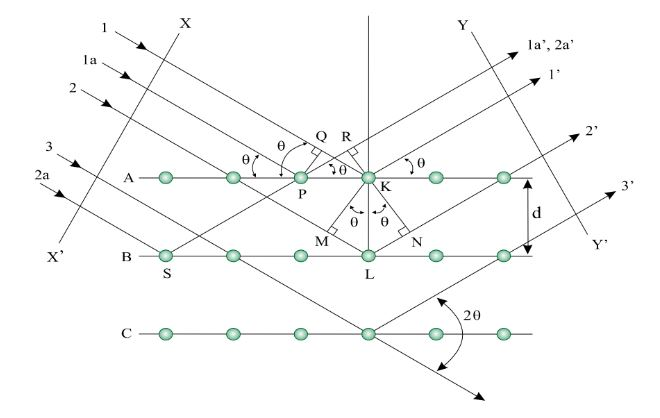
\includegraphics[scale=0.7]{Figuras/leidebragg.jpg}
    \caption{Configuração geométrica da lei de Bragg. Fonte: Adaptada de Cullity [4]}
    \label{fig:ex}
\end{figure}
Importante notar que a lei de Bragg informa dá informações do feixe difratado sem qualquer referência à sua intensidade e que o ângulo entre os feixes incidente e difratado é $2\theta$.

Cada espectro de raios X, comumente denominado de difratograma, é constituído pela superposição do espectro contínuo e da radiação característica.
\begin{figure}[H]
    \centering
    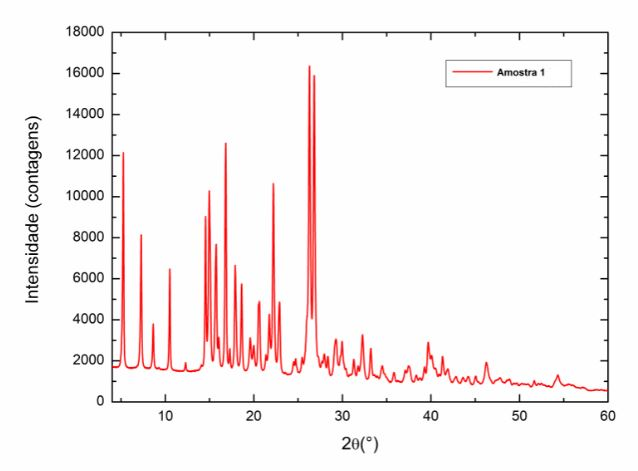
\includegraphics[scale=0.7]{Figuras/ex.jpg}
    \caption{Exemplo de difratograma de uma amostra cristalina. Fonte: elaborada pelos autores.}
    \label{fig:ex}
\end{figure}

\section{Metodologia}
    \subsection{Lista de materiais}
        \begin{itemize}
    \item Aparelho de raios X;
    \item Computador;
    \item Software \textit{X-Ray Apparatus};
    \item \textit{Software Origin};
    \item \textit{Software QTIplot}
    \item Monocristal de \textit{KBr};
    \item Cristal de LiF;
    \item Filtro de \textit{Cu};
    \item Filtro de \textit{Ni}.

\end{itemize}

    \subsection{Montagem experimental}
        O aparato experimental consiste no equipamento de raios X conectado à fonte de alimentação e ao computador. Neste último, o \textit{software X-Ray Apparatus} é aberto para modificar os parâmetros desejados em vez de utilizar diretamente o painel do equipamento. O colimador é responsável por direcionar os raios X, advindos da câmara de raios X, para o alvo localizado na câmara do experimento, onde o goniômetro realiza a varredura do material posicionado no alvo. A figura \ref{fig:aparatoexp} apresenta o aparato experimental utilizado. 
            \begin{figure}[H]
                \centering
                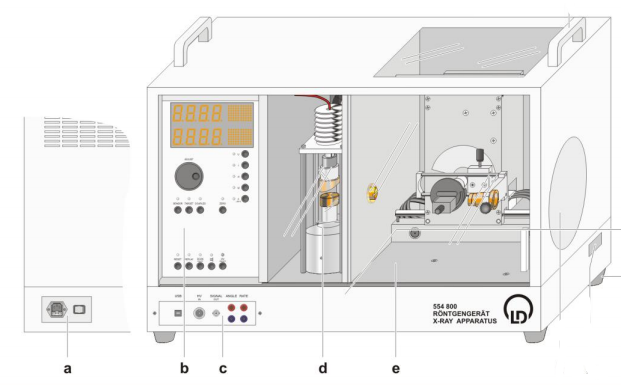
\includegraphics[width=10cm]{aparatoexp.png}
                \caption{Representação do aparato experimental. a – Painel entrada fonte de alimentação; b – Painel de controle; c – Painel de conexão; d – Câmara de Raio-X; e – Câmara do experimento com local para posicionar alvo e goniômetro.}
                \label{fig:aparatoexp}
            \end{figure}
            
        Para o bom andamento do experimento, algumas precauções foram importantes: 
            \renewcommand{\labelenumi}{\roman{enumi}}
                \begin{enumerate}
                    \item  Antes de colocar o aparelho de raios X em operação, foi necessário verificar que a alta tensão estava desligada quando as portas de correr foram abertas (ver \textit{the Instruction Sheet for the x-ray apparatus});
                    \item O acesso ao aparelho de raios X foi restrito a pessoas autorizadas;
                    \item O superaquecimento do anodo Cu do tubo de raios X foi evitado: ao ligar o aparelho de raios X, foi verificado que o ventilador na câmara de tubo estava girando;
                    \item O goniômetro foi posicionado apenas por motores elétricos: o braço do alvo e o braço do sensor do goniômetro não foram bloqueados e não foram movidos manualmente;
                    \item Cristais de NaCl são higroscópicos e extremamente frágeis. O monocristal foi armazenado num lugar seco e manipulado apenas pelas laterias menores, evitando tensões mecânicas ao manipulá-lo.
                \end{enumerate}
                
    \subsection{Procedimento experimental}
        
        O procedimento experimental foi dividido em quatro etapas (1) Lei da Reflexão de Bragg num monocristal de \textit{KBr} utilizando a radiação característica do \textit{Cu}; (2) Cálculo do parâmetro de rede do cristal \textit{LiF}; (3) Análise da borda de absorção de \textit{Ni} e \textit{Cu} e (4) Análise do espectro de energia de um tubo de raios X em função da tensão aplicada. Antes de iniciar o experimento, o nivelamento e o bom funcionamento dos equipamentos foram checados. Não constatando qualquer irregularidade, foi dada  continuidade ao procedimento.
        
            \subsubsection{ Lei da Reflexão de Bragg num monocristal de \textit{KBr} utilizando a radiação característica do \textit{Cu} }
                
                Após a inicialização do \textit{software X-ray Apparatus}, os parâmetros de alta tensão (U), emissão de corrente (\textit{I}), tempo por passo angular ($\Delta$t) e largura por passo angular ($\Delta$$\beta$) foram ajustados da seguinte maneira: U = 35,0 kV, \textit{I} = 1.0 mA, $\Delta$t = 5 s e $\Delta$$\beta$ = 0,1$\degree$ . A tecla \textit{COUPLED} foi pressionada para então definir o valor do limite angular inferior e superior em 5$\degree$  e 48$\degree$ , respectivamente e, ,por fim, o botão \textit{SCAN} foi pressionado para iniciar a medição e transmissão de dados para o computador. A medição durou cerca de 30 minutos e, após a finalização, os dados foram salvos para análise posterior utilizando o \textit{software Origin}.
        
            \subsubsection{Cálculo do parâmetro de rede do cristal \textit{LiF}}
                O procedimento experimental desta etapa é análogo ao da etapa anterior, diferenciando-se apenas no limite angular inferior e superior de 10$\degree$  e 25$\degree$ , respectivamente. Todos os demais parâmetros permanecem inalterados: U = 35,0 kV, \textit{I} = 1.0 mA, $\Delta$t = 5 s e $\Delta$$\beta$ = 0,1$\degree$. 
            
            \subsubsection{Análise da borda de absorção de \textit{Ni} e \textit{Cu}}
                Nesta etapa, filtros foram posicionados no \textit{sensor seat} do goniômetro. A primeira medição foi realizada utilizando o filtro de \textit{Cu} e ajustando os parâmetros da seguinte forma: U = 35,0 kV, \textit{I} = 1.0 mA, $\Delta$t = 5 s e $\Delta$$\beta$ = 0,1$\degree$.
                
                A tecla \textit{COUPLED} foi pressionada para então definir o valor do limite angular inferior de 10$\degree$  e superior de 25$\degree$  e, por fim, o botão \textit{SCAN} foi pressionado para iniciar a medição e transmissão de dados para o computador. A medição durou cerca de 15 minutos. O mesmo procedimento foi feito utilizando o filtro de \textit{Ni}.
                
            \subsubsection{Análise do espectro de energia de um tubo de Raios X em função da tensão aplicada}
            
                A última etapa do experimento foi dada pela variação das tensões fixando os demais parâmetros - \textit{I} = 100 mA, $\Delta$t = 10 s e $\Delta$$\beta$ = 0,1$\degree$ e limite angular inferior e superior de 10$\degree$ e 25$\degree$, respectivamente. A tensão foi fixada em U = 10kV. Assim, a medição foi iniciada e e transferência de dados para o computador foi feita pressionando o comando \textit{SCAN}. 
                O procedimento foi repetido para diferentes valores de tensão: 15 kV, 20 kV, 25kV e 30kV, em que cada medição durou cerca de 30 minutos.

                
        
    
\section{Resultados e análise de dados}

\subsection{Comprimento de onda dos raios X de cobre}

No gráfico \label{fig:kbr} é exibido o difratograma seguido da tabela \ref{tab:kbr} que apresenta a localização dos picos para a primeira etapa desse experimento. 

\begin{figure}[H]
    \centering
    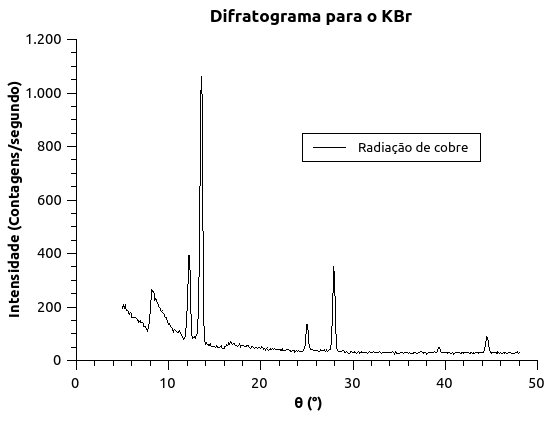
\includegraphics[scale=0.8]{Figuras/KBr_cu.png}
    \caption{Picos de intensidade para uma radiação do cobre incidindo sobre uma amostra de brometo de potássio.}
    \label{fig:kbr}
\end{figure}

\begin{table}[H]
    \centering
    \caption{Ordem da difração e localização dos picos em $\theta$ para cada tipo de radiação.}
    \begin{tabular}{|c|c|c|}
        \hline
         n & $\theta$ $[K_\alpha]$ $(^o)$ & $\theta$ $[K_\beta]$ $(^o)$ \\ \hline
         1 & $13,52\pm0,14$ & $12,19\pm0,14$ \\ \hline
         2 & $27,91\pm0,14$ & $25,00\pm0,13$ \\ \hline
         3 & $44,52\pm0,14$ & $39,31\pm0,10$ \\ \hline
    \end{tabular}
    \label{tab:kbr}
\end{table}

Tendo esses dados, foi traçado os gráficos $n \times \sin(\theta)$ apresentados nas figuras \ref{fig:kbr-ka} e \ref{fig:kbr-kb} a fim de se obter o comprimento de onda médio à partir do coeficiente angular do ajuste linear.

\begin{figure}[H]
    \centering
    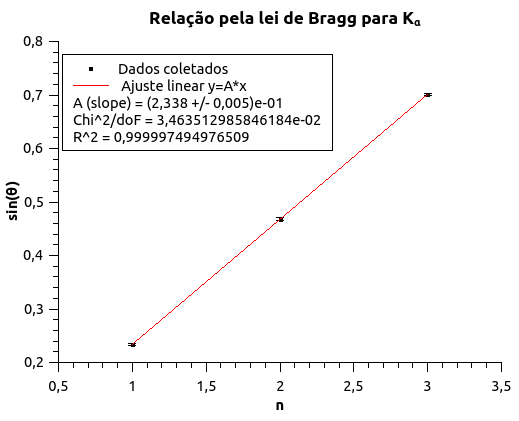
\includegraphics[scale=0.8]{Figuras/Ka.png}
    \caption{Ajuste linear para a radiação $K_\alpha$}
    \label{fig:kbr-ka}
\end{figure}

\begin{figure}[H]
    \centering
    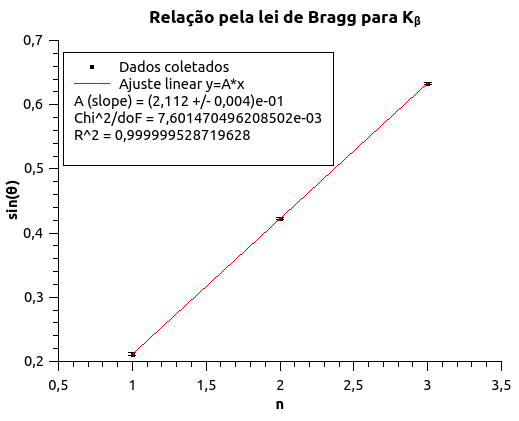
\includegraphics[scale=0.8]{Figuras/Kb.png}
    \caption{Ajuste linear para a radiação $K_\beta$}
    \label{fig:kbr-kb}
\end{figure}

Assim, foi possível obter os comprimentos de onda:
$$\lambda_{K\alpha}=2dA_\alpha=(1,542\pm0,003)\text{\normalfont\AA}$$
$$\lambda_{K\beta}=2dA_\beta=(1,393\pm0,003)\text{\normalfont\AA}$$
e os erro relativo para cada valor obtido:
$$E_\alpha=\frac{|1,54180-1,542|}{1,54180}=0,01\%$$
$$E_\beta=\frac{|1,39342-1,393|}{1,39342}=0,03\%$$

\subsection{Parâmetro de rede do cristal de LiF}

O difratograma e a localização dos picos para o cristal de LiF são apresentados, respectivamente, na figura \ref{fig:LiF} e na tabela \ref{tab:dLiF} abaixo.

\begin{figure}[H]
    \centering
    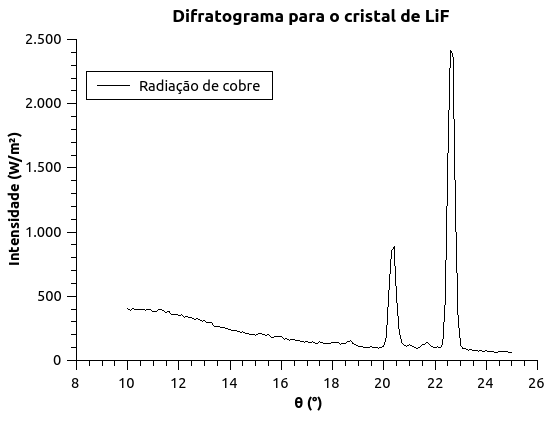
\includegraphics[scale=0.8]{Figuras/LiF.png}
    \caption{Picos de intensidade para a difração do LiF com radiação de cobre.}
    \label{fig:LiF}
\end{figure}

\begin{table}[H]
    \centering
    \caption{Localização em $\theta$ dos picos de intensidade de difração para o LiF com radiação de cobre.}
    \begin{tabular}{|c|c|}
        \hline
        $\theta$ $[K_\alpha]$ $(^o)$ & $22,64\pm0,12$ \\ \hline
        $\theta$ $[K_\beta]$ $(^o)$ & $20,35\pm0,11$ \\ \hline
    \end{tabular}
    \label{tab:dLiF}
\end{table}

Por fim os resultados são exibidos na tabela \ref{tab:LiF}.

\begin{table}[H]
    \centering
    \caption{Resultados obtidos para a distância interplanar $d$ e o parâmetro de rede $a_0$.}
    \begin{tabular}{|c|c|c|}
        \hline
        n=1 & $d$ (\r{A}) & $a_0$ (\r{A}) \\ \hline
        $K_\alpha$ & $2,00\pm0,01$ & $4,01\pm0,02$ \\ \hline
        $K_\beta$ & $2,00\pm0,01$ & $4,01\pm0,02$ \\ \hline
        Valor médio & $2,00\pm0,01$ & $4,01\pm0,02$ \\ \hline
        Valor na literatura & 2,015 & 4,03 \\ \hline
    \end{tabular}
    \label{tab:LiF}
\end{table}

Os erros relativos são então
$$E_d=\frac{|2,015-2,00|}{2,015}=0,7\%$$
$$E_{a0}=\frac{|4,03-4,01|}{4,03}=0,5\%$$

\subsection{Filtros}

\begin{figure}[H]
    \centering
    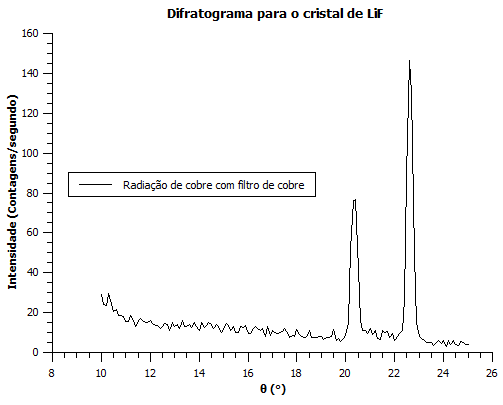
\includegraphics[scale=0.8]{Figuras/FiltroCu.png}
    \caption{Caption}
    \label{fig:my_label}
\end{figure}

\begin{figure}[H]
    \centering
    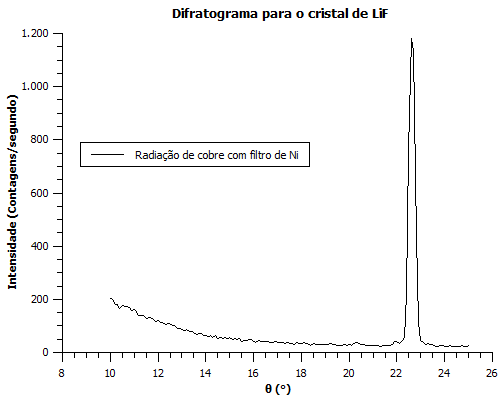
\includegraphics[scale=0.8]{Figuras/FiltroNi.png}
    \caption{Caption}
    \label{fig:my_label}
\end{figure}


\begin{figure}[H]
    \centering
    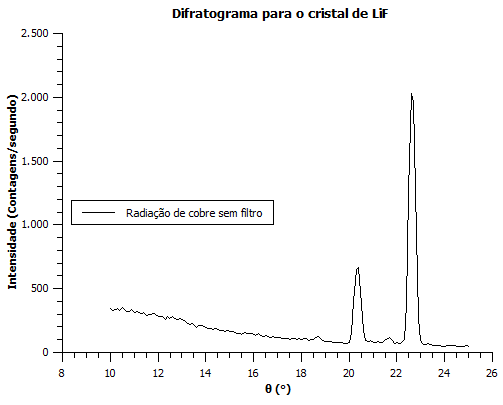
\includegraphics[scale=0.8]{Figuras/Semfiltro.png}
    \caption{Caption}
    \label{fig:my_label}
\end{figure}

\begin{table}[H]
    \centering
    \begin{tabular}{|c|c|c|}
        \hline
        Filtro & Radiação & $\theta(^o)$ \\ \hline
        Cu & $K_\alpha$ & $22,63\pm0,11$ \\ \hline
        Cu & $K_\beta$ & $20,35\pm0,10$ \\ \hline
        Ni & $K_\alpha$ & $22,63\pm0,11$ \\ \hline
        Sem filtro & $K_\alpha$ & $22,64\pm0,11$ \\ \hline
        Sem filtro & $K_\beta$ & $20,35\pm0,12$ \\ \hline
    \end{tabular}
    \caption{Com filtro - Cu}
    \label{tab:my_label4}
\end{table}

\begin{table}[H]
    \centering
    \begin{tabular}{|c|c|c|c|c|}
    \hline
         & $R(K_\alpha)$ & $R(K_\beta)$ & $V_0$ & $V$ \\ \hline
        Sem filtro & 2413,8 & 885,6 & 0,36689038 & 0,268412439 \\ \hline
        Filtro de Cu & 146,2 & 76,8 & 0,525307798 & 0,344394619 \\ \hline
        Filtro de Ni & 1.182 & 0 & 0 & 0 \\ \hline 
    \end{tabular}
    \caption{Caption}
    \label{tab:my_label}
\end{table}

\subsection{exp 2}

\begin{table}[H]
    \centering
    \begin{tabular}{|c|c|c|c|}
        \hline
        10kV & $\theta$ $[K_\alpha]$ $(^o)$ & $22,53\pm0,10$ & 1.544\\ \hline
        10kV & $\theta$ $[K_\beta]$ $(^o)$ & $20,26\pm0,11$ & 1.396\\ \hline
        15kV & $\theta$ $[K_\alpha]$ $(^o)$ & $22,53\pm0,10$ & 1.544\\ \hline
        15kV & $\theta$ $[K_\beta]$ $(^o)$ & $20,26\pm0,10$ & 1.396\\ \hline
        20kV & $\theta$ $[K_\alpha]$ $(^o)$ & $22,53\pm0,10$ & 1.544\\ \hline
        20kV & $\theta$ $[K_\beta]$ $(^o)$ & $20,25\pm0,10$ & 1.395\\ \hline
        25kV & $\theta$ $[K_\alpha]$ $(^o)$ & $22,54\pm0,11$ & 1.545\\ \hline
        25kV & $\theta$ $[K_\beta]$ $(^o)$ & $20,26\pm0,11$ & 1.396\\ \hline
        30kV & $\theta$ $[K_\alpha]$ $(^o)$ & $22,54\pm0,11$ & 1.545\\ \hline
        30kV & $\theta$ $[K_\beta]$ $(^o)$ & $20,26\pm0,10$ & 1.396\\ \hline
    \end{tabular}
    \caption{LiF}
    \label{tab:my_label7}
\end{table}

\section{Conclusão}

\appendix

\newpage

\bibliographystyle{abntex2-num}
\bibliography{refs.bib}

\nocite{*}

\section{Demonstrações}

\section{Propagação de incertezas}

\subsection{Distância d entre planos cristalinos}
$$d=\frac{\lambda}{2\sin(\theta)}$$
$$\sigma_d=\sqrt{\qty(\pdv{d}{\lambda}\sigma_\lambda)^2+\qty(\pdv{d}{\theta}\sigma_\theta)^2}=\sqrt{\qty(\frac{1}{2\sin(\theta)}\sigma_\lambda)^2+\qty(-\frac{\lambda}{2\sin(\theta)\tan(\theta)}\sigma_\theta)^2}$$
$$\sigma_d=d\sqrt{\qty(\frac{\sigma_\lambda}{\lambda})^2+\qty(\frac{\sigma_\theta}{\tan(\theta)})^2}$$

\end{document}